\documentclass{article}
\usepackage[UTF8]{ctex}
\usepackage{amsmath,mathtools,geometry,caption,tikz,float}
\geometry{a4paper,scale=0.7}

\title{每日一题(13.2)}
\author{\kaishu 李政毅、程昊一}
\date{2022年4月6日}

\begin{document}
\maketitle
\textbf{1. }如图, $DE\parallel BC$, $BF$平分$\angle ABC$, 交$DE$于$F$, 且$BD+CE=DE$. 求证: $CF$平分$\angle ACB$.\\
\rightline{\kaishu(李政毅供题)}
\begin{figure}[H]
	\centering
	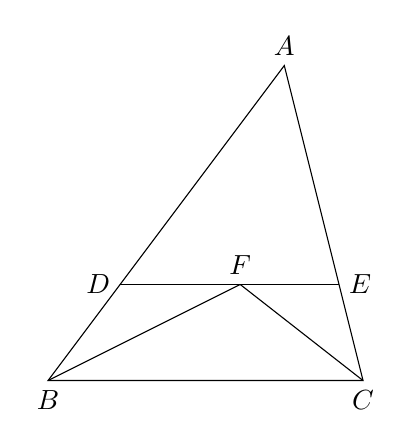
\begin{tikzpicture}
		\node at (3,4) [above] {$A$};
		\node at (0,0) [below] {$B$};
		\node at (4,0) [below] {$C$};
		\node at (0.91,1.22) [left] {$D$};
		\node at (3.7,1.22) [right] {$E$};
		\node at (2.44,1.22) [above] {$F$};
		
		\draw (3,4)--(0,0)--(4,0)--cycle;
		\draw (0,0)--(2.44,1.22);
		\draw (2.44,1.22)--(4,0);
		\draw (0.91,1.22)--(3.7,1.22);
	\end{tikzpicture}
	\caption*{\kaishu 第一题图}
\end{figure}\par
\textbf{2. }如图, $AA'$, $BB'$分别平分$\angle EAB$, $\angle DBC$. 若$AA'=BB'=AB$, 求$\angle BAC$.\\
\rightline{\kaishu(程昊一供题)}
\begin{figure}[H]
	\centering
	\begin{tikzpicture}
		\node at (0,0) [above] {$A$};
		\node at (2.5,0) [below] {$B$};
		\node at (3.09,0.66) [above] {$C$};
		\node at (4,0) [right] {$D$};
		\node at (-0.63,-0.13) [left] {$E$};
		\node at (0.26,-2.49) [below] {$A'$};
		\node at (4.78,1.02) [right] {$B'$};
		
		\draw (0,0)--(0.26,-2.49)--(2.5,0)--(4.78,1.02)--cycle;
		\draw (0,0)--(4,0);
		\draw (2.5,0)--(3.09,0.66);
		\draw (0,0)--(-0.63,-0.13);
	\end{tikzpicture}
	\caption*{\kaishu 第二题图}
\end{figure}
\end{document}